\documentclass[12pt, a4paper]{report}
\usepackage[pdftex]{graphicx} %for embedding images
\graphicspath{ {./img/} } %the path to the images
\usepackage[,italian, english]{babel}
\usepackage{url} %for proper url entries
% \usepackage[bookmarks, colorlinks=false, pdfborder={0 0 0}, pdftitle={<pdf title here>}, pdfauthor={<author's name here>}, pdfsubject={<subject here>}, pdfkeywords={<keywords here>}]{hyperref} %for creating links in the pdf version and other additional pdf attributes, no effect on the printed document
%\usepackage[final]{pdfpages} %for embedding another pdf, remove if not required
%pseudocode listing packages and definitions
\usepackage{color}
\usepackage{listings}
\usepackage{caption}

\newcounter{nalg}[chapter] % defines algorithm counter for chapter-level
\renewcommand{\thenalg}{\thechapter .\arabic{nalg}} %defines appearance of the algorithm counter
\DeclareCaptionLabelFormat{algocaption}{Algorithm \thenalg} % defines a new caption label as Algorithm x.y

\lstnewenvironment{algorithm}[1][] %defines the algorithm listing environment
{   
    \refstepcounter{nalg} %increments algorithm number
    \captionsetup{labelformat=algocaption,labelsep=colon} %defines the caption setup for: it ises label format as the declared caption label above and makes label and caption text to be separated by a ':'
    \lstset{ %this is the stype
        mathescape=true,
        frame=tB,
        numbers=left, 
        numberstyle=\tiny,
        basicstyle=\scriptsize, 
        keywordstyle=\color{black}\bfseries\em,
        keywords={,input, output, return, datatype, function, in, if, else, foreach, while, begin, end, } %add the keywords you want, or load a language as Rubens explains in his comment above.
        numbers=left,
        xleftmargin=.04\textwidth,
        #1 % this is to add specific settings to an usage of this environment (for instnce, the caption and referable label)
    }
}
{}

\begin{document}
\renewcommand\bibname{References} %Renames "Bibliography" to "References" on ref page


\begin{titlepage}

\begin{center}

\Large \textbf {Programmazione Concorrente e Distribuita - Assigment 03 - Part 1}\\%\\[0.5in]
\vspace{1em}%
\vfill
Andrea Biagini


Filippo Gurioli


Leonardo Randacio
\vspace{1em}
\vfill
{\bf Università di Bologna \\ Scienze e Ingegneria Informatiche}\\[0.5in]

       
\vfill
\today

\end{center}

\end{titlepage}


\tableofcontents

\newpage
\pagenumbering{arabic} %reset numbering to normal for the main content

The part 1 was created modifing the Assignment-01. The report is reported fully, with meaningfull changes in architecture and implementation.

\chapter{Analysis}
The goal is to create a concurrent agent-based simulation.

An agent-based simulation or model is a computational modeling
 technique used to simulate complex systems by representing individual
 entities, known as agents, and their interactions within an environment.
 The goal of the simulation is to observe the evolution of the states of the
 environment and the agents in each discrete step.

Agents beheviour for a single step can be described in 3 phases:
\begin{itemize}
   \item sense phase: the agent acquires data from the environment
   \item decide phase: the agent determines the next action
   \item act phase: the action determined is executed on the environment
\end{itemize}

\section{Task Decomposition}
Each agent's step can compose a single task, which can be divided into 3 subtasks,
 one for each phase of the step. 

This means that for a given step there will be 3 tasks:
\begin{itemize}
    \item sense
    \item decide
    \item act
\end{itemize}

The total number of tasks for a given step is 3 * nAgents
 where nAgents is the number of agents.

\section{Data Decomposition}
The environment can be subdevided in agent's states which
 means the data can be divided in nAgents indipendent states.

\section{Dependency Analysis}
The sense and decide tasks can be joined in a single
 sense-decide task as the sense task only quearies the
 environment and the decide task updates the next action
 to be performed for a given agent. Since the decide phase
 only sets the next action for a given agent and for a
 given step every agent's next action will be set only
 by one decide task, the sense-decide tasks can be executed
 in a concurrent manner.

The act tasks in a given step can be parallelised between each other, but
 must be executed after the sense-decide task.

The steps of the simulation must be serialized.

\chapter{Design}
Using agenda parallelism we design the system around an agenda
 composed by the various tasks, which were defined earlier. Every
 step in the simulation imposes a mandatory syncronization.

Using the actors concurrency one actor will be initialized for every agent in the simulation.

\section{Architecture}
A simulation will present an actor for every agent present. The syncronization of the agents will be obtained by a "simulation" actor,
 which will behave similarly to a master in a master-slave architecture, ensuring the correct execution and ordering of the various steps.

Also actors will rappresent various views, that will be able to communicate with the "simulation" actor, ensuring timely updates and interactions.

The "simulation" actor will also keep track of the overall state of the simulation.
\section{Visual Formalisms}

To rappresent an exemplary run of the simulation a sequence diagram has been choosen. The lifelines where omitted as they are trivial. All the arrows
 rappresent asyncronous messages as for the actor architecture. The arrows are rappresented with open arrowheads to enphasize the asyncronous nature of
 communication.

A simulation runner is also rappresented as the main actor and first to be initialized.

\begin{figure}
    \centering
    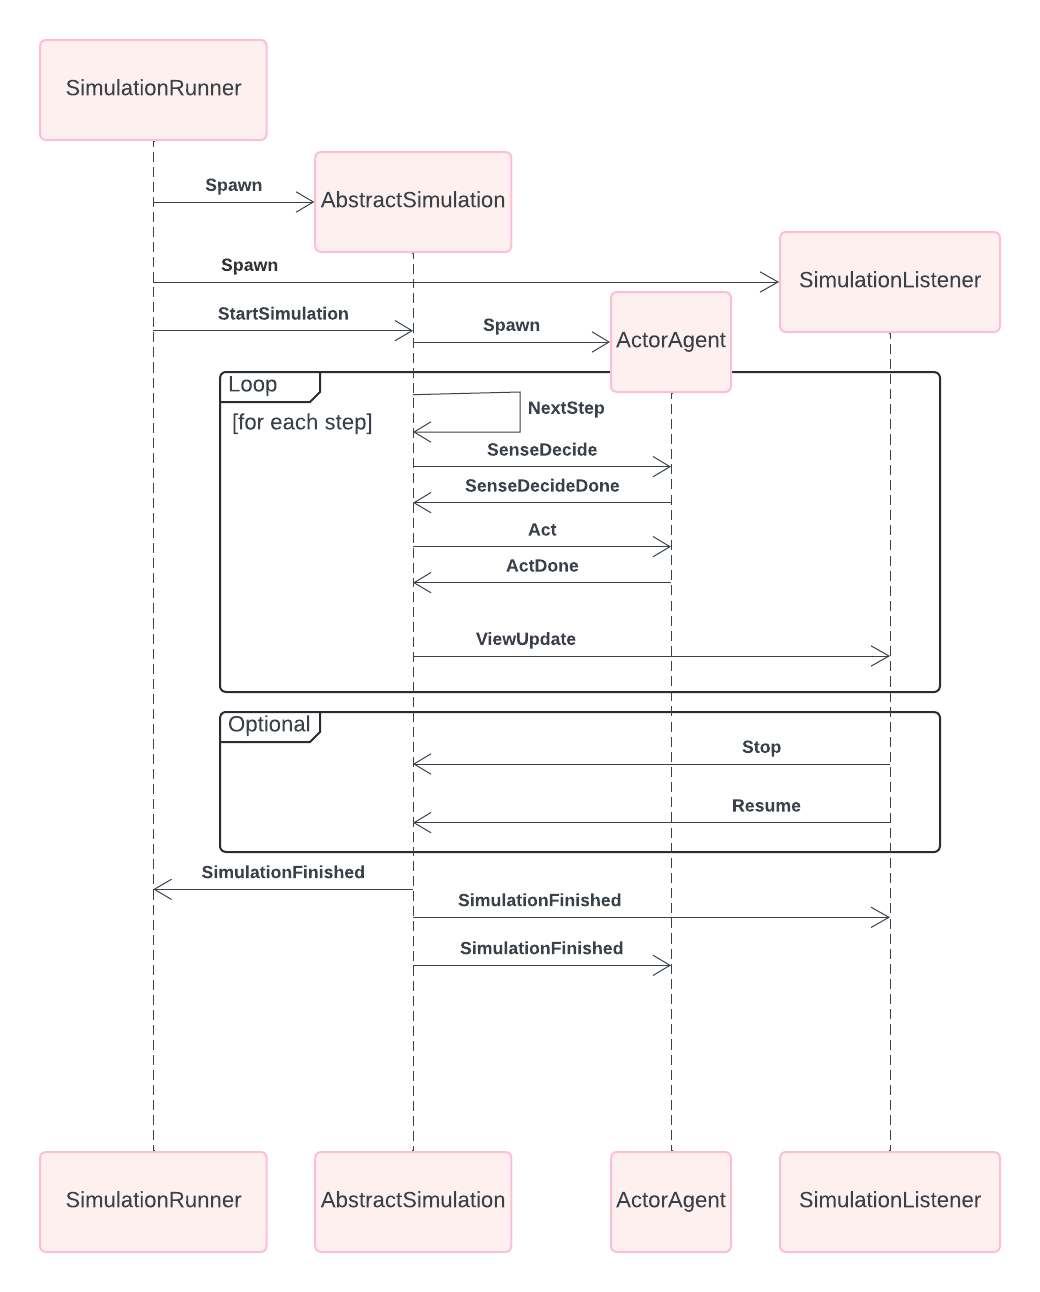
\includegraphics{actorsSD.png}
    \caption{Sequence diagram of the system.}
\end{figure}

\newpage

\chapter{Implementation}

Java akka typed actors have been used to implement the actor architecture.

\section{Source Code Organization}
The basic simulation implementation has been extended with the GUI implementation.

The GUI source code is comprised of only one class: simtrafficexamplesconcurrent/RoadSimView.java.

The class simtrafficexamplesconcurrent/RoadSimView.java prints information of the simulation on the terminal.

The src is organized in the following packages:
\begin{itemize}
    \item actor: containing classes for the actor agents and utilities for the actors of the system.
    \item simengine: abstract classes for the simulation framework.
    \item simtrafficbase: concrete classes for the traffic simulation.
    \item simtrafficexamples: concrete simulation and main classes given as examples.
\end{itemize}

\chapter{Execution and Evaluation}

The main classes are contained in the \texttt{simtrafficexamples} package.

\begin{itemize}
    \item \texttt{RunTrafficSimulation.java}: some simple examples of traffic simulations
    \item \texttt{RunMassiveTrafficSimulation.java}: a simulation with a massive number of cars
\end{itemize}

\chapter{Conclusions}

The akka library has shown to be very powerfull but has not shown to be easy to use. Combining the abstraction requirements of the assignment with the
 akka typed actors synctax has proven challenging at times, requiring advanced programming (see \emph{create()} method in the \emph{AbstractSimulation.java} file).

Although the utilization of the library was initially not perceived as intuitive; however, after comprehending the foundational syntax and implementation,
 the execution of the assignment proceeded seamlessly.

The actor pattern has proven to be very powerfull, also given the fact that it rappresents a direct ancestor of the agent pattern showcased in the assignment.

\section{Improvements}
The current implementation might be considered to be partially violating the actor pattern as the actors rappresenting the single agents execute methods
 directly on the data structures contained in the simulation actor. This could be replaced by a more sound message protocol, where messages from the
 simulation to the actor agents contain the informations on the current state of the environment and the agents response contain the updated environment
 acted upon by the agents. This could prove to be hard to implement while maintaing the required abstraction as contents of these type of messages would
 depend on the concrete version of the simulation and would change from simulation to simulation.

\bibliographystyle{plain}
\bibliography{References}

\end{document}